\documentclass[11pt,a4paper]{article}
\usepackage[utf8]{inputenc}
\usepackage[spanish]{babel}
\usepackage{amsmath}
\usepackage{amsfonts}
\usepackage{amssymb}
\usepackage{graphicx}
\usepackage{caption}
\captionsetup[table]{name=Tabla}
\date{}
\usepackage{float}
\usepackage[left=2cm,right=2cm,top=2cm,bottom=2cm]{geometry}
\title{Elección de centros}
\begin{document}
\textbf{Primer ejemplo: EDP 1}
\begin{figure}[H]
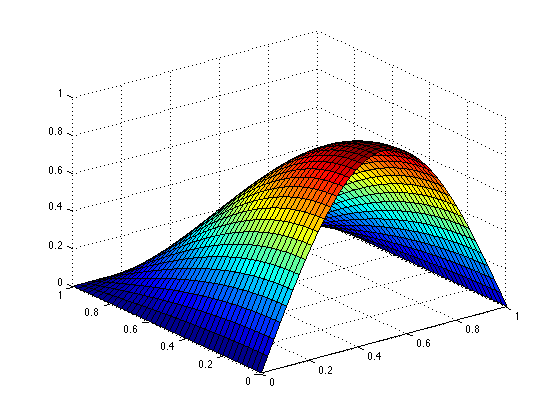
\includegraphics[scale=.5]{edp1.png}
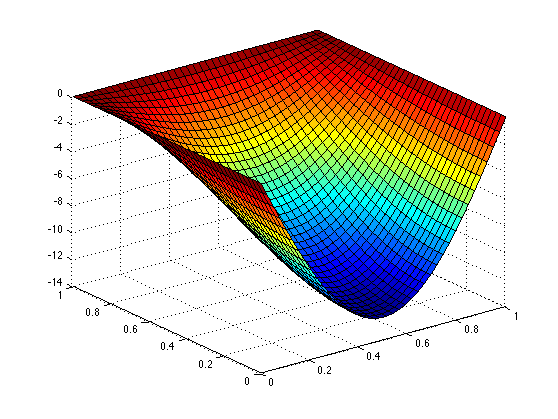
\includegraphics[scale=.4]{Ledp1.png}
\caption{Solución de la primera EDP y operador aplicado a la solución.}
\end{figure}
Distribución inicial de centros: 
\begin{figure}[H]
\begin{center}
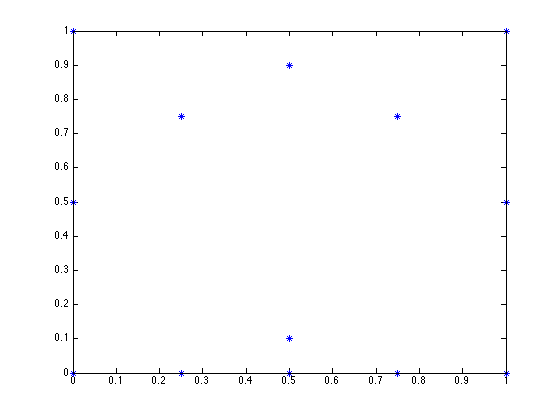
\includegraphics[scale=.5]{inicial1.png}
\caption{Distribución inicial de centros.}
\end{center}
\end{figure}


\begin{table}[H]
\caption{Resultados readaptando el parámetro de forma.}
\begin{center}
\begin{tabular}{|c|c|c|c|c|c|c|}
\hline
\ Tol & ECM & N & $D_{min}$ & Cond  & iter \\
\hline
\ $10^{-1}$ & 1.0912e-02 & 14 & 5.0000e-02 & 2.7562e+07 &  2\\
\ $10^{-2}$ & 1.6256e-03 &25 & 2.5000e-02& 9.0759e+10 & 3 \\
\ $10^{-3}$& 7.5254e-05& 39 & 2.5000e-02 &  8.2675e+14 &  3 \\
\ $10^{-4}$& 8.9124e-06& 79 & 6.2500e-03 &  2.4175e+18 &  5 \\
\ $10^{-5}$& 3.9562e-05& 1301 & 6.2500e-03 & 3.2166e+20 &  5 \\
\hline
\end{tabular}
\end{center}
\end{table}

\begin{figure}[H]
\begin{center}
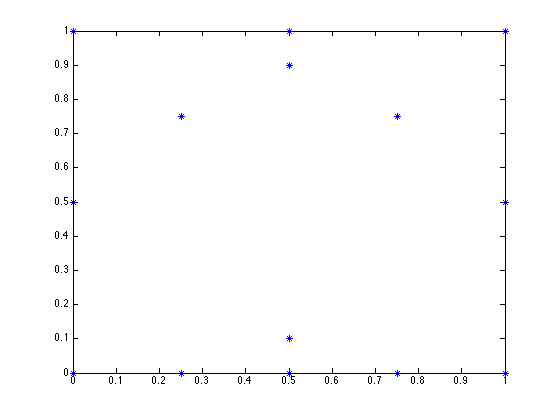
\includegraphics[scale=.4]{edp1_tol1.png}
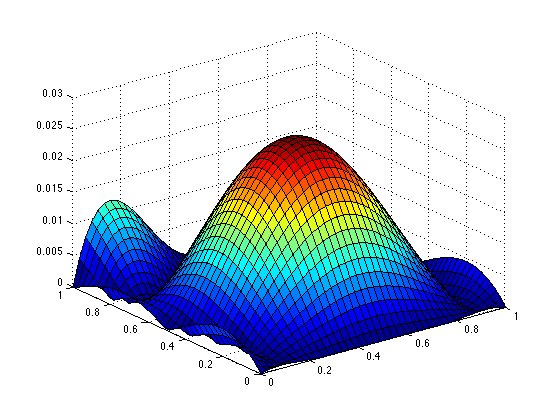
\includegraphics[scale=.4]{error_edp1_tol1.png}
\caption{Distribución de centros y del error con tolerancia $10^{-1}$}
\end{center}
\end{figure}

\begin{figure}[H]
\begin{center}
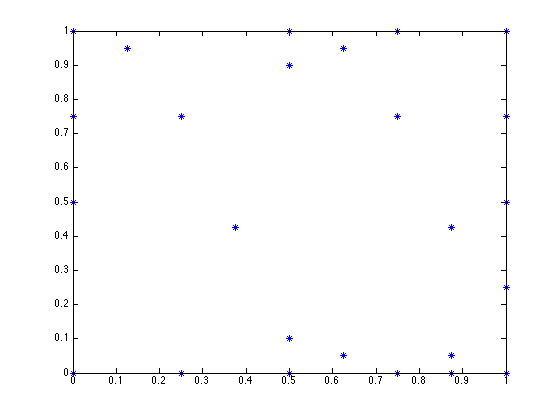
\includegraphics[scale=.4]{edp1_tol2.png}
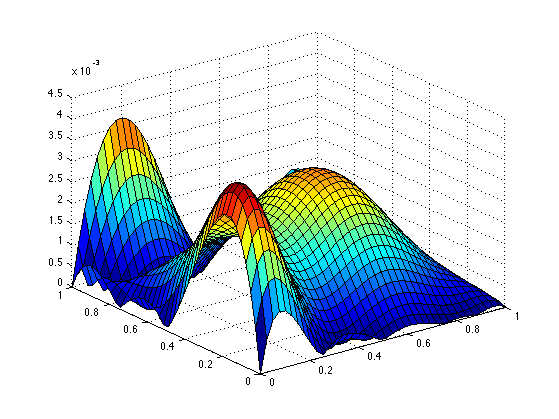
\includegraphics[scale=.4]{error_edp1_tol2.png}
\caption{Distribución de centros y del error con tolerancia $10^{-2}$}
\end{center}
\end{figure}

\begin{figure}[H]
\begin{center}
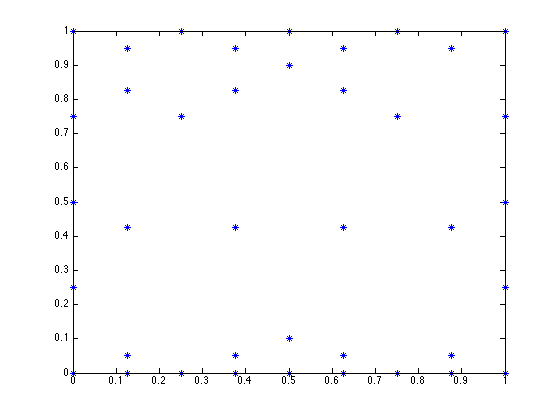
\includegraphics[scale=.4]{edp1_tol3.png}
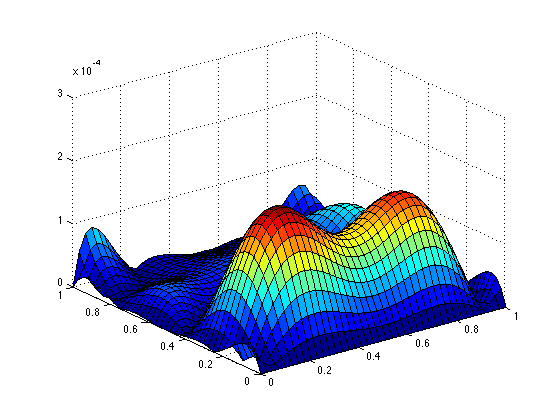
\includegraphics[scale=.4]{error_edp1_tol3.png}
\caption{Distribución de centros y del error con tolerancia $10^{-3}$}
\end{center}
\end{figure}

\begin{figure}[H]
\begin{center}
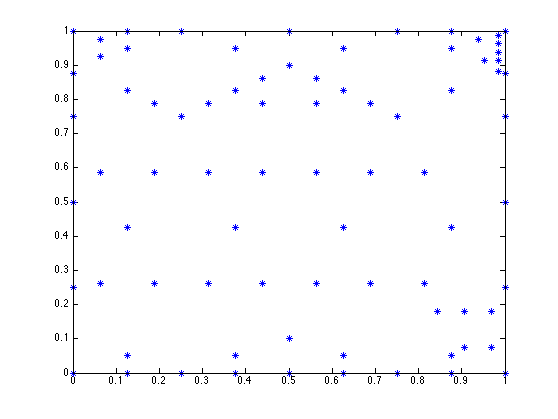
\includegraphics[scale=.4]{edp1_tol4.png}
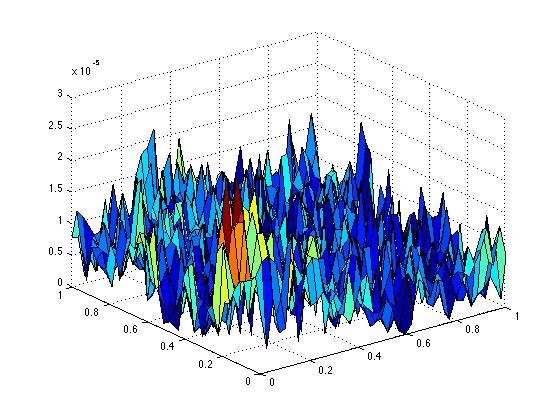
\includegraphics[scale=.4]{error_edp1_tol4.png}
\caption{Distribución de centros y del error con tolerancia $10^{-4}$}
\end{center}
\end{figure}

\begin{figure}[H]
\begin{center}
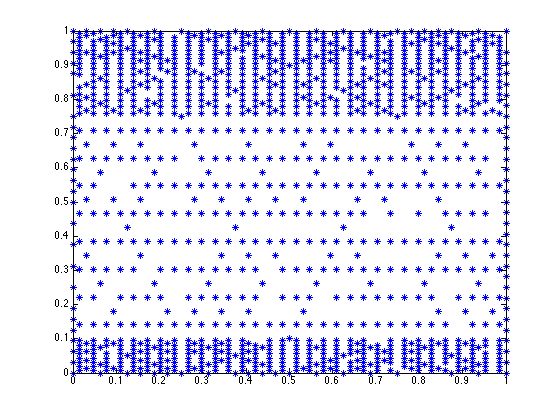
\includegraphics[scale=.4]{edp1_tol5.png}
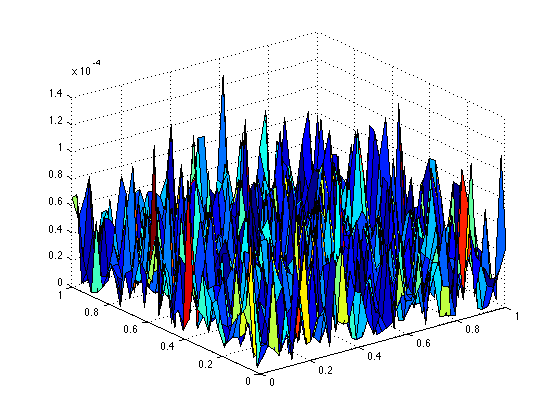
\includegraphics[scale=.4]{error_edp1_tol5.png}
\caption{Distribución de centros y del error con tolerancia $10^{-5}$}
\end{center}
\end{figure}


 \newpage
\textbf{Segundo ejemplo: edp 3}
\begin{figure}[H]
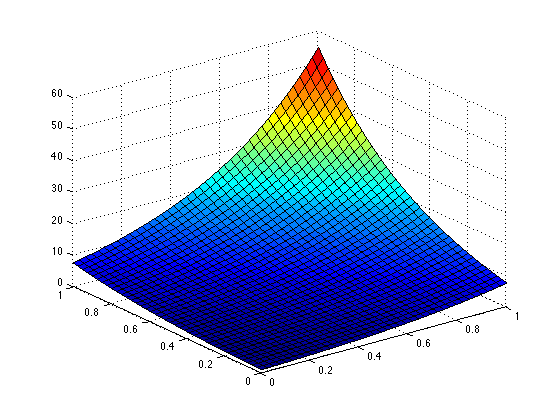
\includegraphics[scale=.45]{edp3.png}
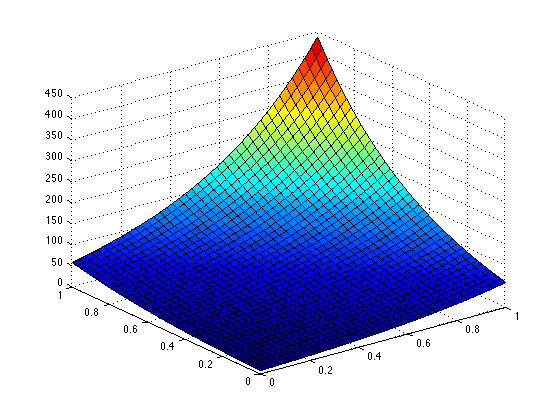
\includegraphics[scale=.45]{Ledp3.png}
\caption{Solución de la primera EDP y operador aplicado a la solución.}
\end{figure}

Distribución inicial de centros: 
\begin{figure}[H]
\begin{center}
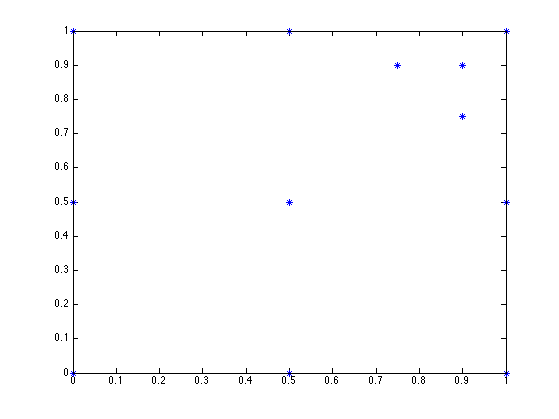
\includegraphics[scale=.5]{inicial2.png}
\caption{Distribución inicial de centros.}
\end{center}
\end{figure}

\begin{table}[H]
\caption{Resultados readaptando el parámetro de forma.}
\begin{center}
\begin{tabular}{|c|c|c|c|c|c|c|}
\hline
\ Tol & ECM & N & $D_{min}$ & Cond  & iter \\
\hline
\ $10^{-1}$ & 2.3707e-03& 115&6.2500e-03 &1.4330e+16  &  5\\
\ $10^{-2}$ & 3.7685e-04 &341 &6.2500e-03  &1.6213e+19 & 5 \\
\ $10^{-3}$&3.7410e-04 &1326 &6.2500e-03  & 4.8270e+20 &  5 \\

\hline
\end{tabular}
\end{center}
\end{table}

\begin{figure}[H]
\begin{center}
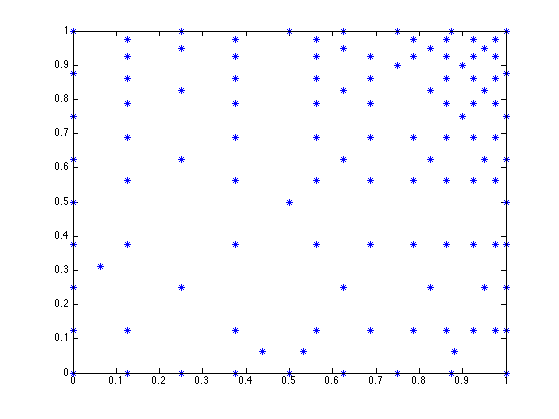
\includegraphics[scale=.4]{edp3_tol1.png}
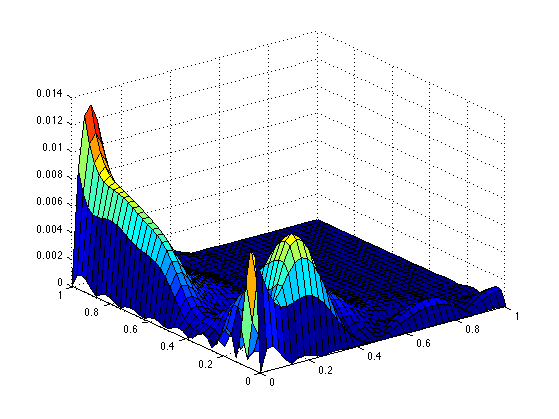
\includegraphics[scale=.4]{error_edp3_tol1.png}
\caption{Distribución de centros y del error con tolerancia $10^{-1}$}
\end{center}
\end{figure}

\begin{figure}[H]
\begin{center}
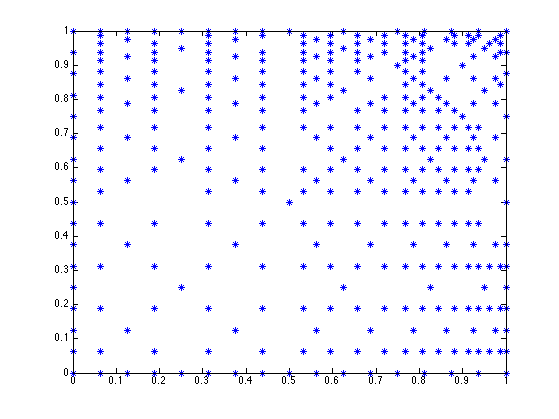
\includegraphics[scale=.4]{edp3_tol2.png}
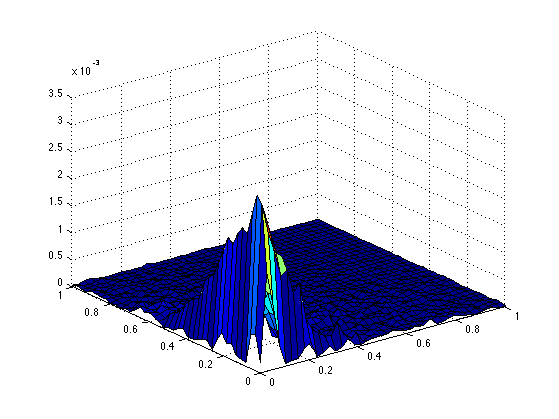
\includegraphics[scale=.4]{error_edp3_tol2.png}
\caption{Distribución de centros y del error con tolerancia $10^{-2}$}
\end{center}
\end{figure}

\begin{figure}[H]
\begin{center}
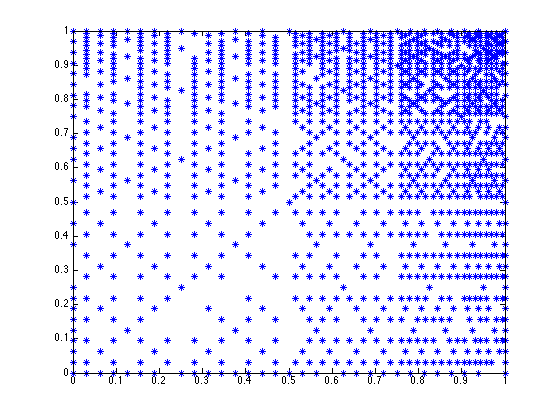
\includegraphics[scale=.4]{edp3_tol3.png}
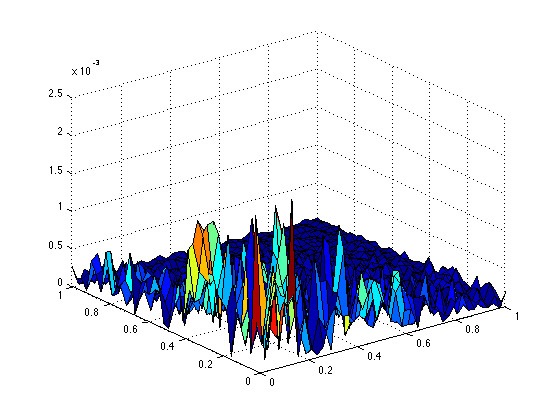
\includegraphics[scale=.4]{error_edp3_tol3.png}
\caption{Distribución de centros y del error con tolerancia $10^{-3}$}
\end{center}
\end{figure}


\end{document}

